\pgfdeclareplotmark{cross} {
\pgfpathmoveto{\pgfpoint{-0.3\pgfplotmarksize}{\pgfplotmarksize}}
\pgfpathlineto{\pgfpoint{+0.3\pgfplotmarksize}{\pgfplotmarksize}}
\pgfpathlineto{\pgfpoint{+0.3\pgfplotmarksize}{0.3\pgfplotmarksize}}
\pgfpathlineto{\pgfpoint{+1\pgfplotmarksize}{0.3\pgfplotmarksize}}
\pgfpathlineto{\pgfpoint{+1\pgfplotmarksize}{-0.3\pgfplotmarksize}}
\pgfpathlineto{\pgfpoint{+0.3\pgfplotmarksize}{-0.3\pgfplotmarksize}}
\pgfpathlineto{\pgfpoint{+0.3\pgfplotmarksize}{-1.\pgfplotmarksize}}
\pgfpathlineto{\pgfpoint{-0.3\pgfplotmarksize}{-1.\pgfplotmarksize}}
\pgfpathlineto{\pgfpoint{-0.3\pgfplotmarksize}{-0.3\pgfplotmarksize}}
\pgfpathlineto{\pgfpoint{-1.\pgfplotmarksize}{-0.3\pgfplotmarksize}}
\pgfpathlineto{\pgfpoint{-1.\pgfplotmarksize}{0.3\pgfplotmarksize}}
\pgfpathlineto{\pgfpoint{-0.3\pgfplotmarksize}{0.3\pgfplotmarksize}}
\pgfpathclose
\pgfusepathqstroke
}
\pgfdeclareplotmark{cross*} {
\pgfpathmoveto{\pgfpoint{-0.3\pgfplotmarksize}{\pgfplotmarksize}}
\pgfpathlineto{\pgfpoint{+0.3\pgfplotmarksize}{\pgfplotmarksize}}
\pgfpathlineto{\pgfpoint{+0.3\pgfplotmarksize}{0.3\pgfplotmarksize}}
\pgfpathlineto{\pgfpoint{+1\pgfplotmarksize}{0.3\pgfplotmarksize}}
\pgfpathlineto{\pgfpoint{+1\pgfplotmarksize}{-0.3\pgfplotmarksize}}
\pgfpathlineto{\pgfpoint{+0.3\pgfplotmarksize}{-0.3\pgfplotmarksize}}
\pgfpathlineto{\pgfpoint{+0.3\pgfplotmarksize}{-1.\pgfplotmarksize}}
\pgfpathlineto{\pgfpoint{-0.3\pgfplotmarksize}{-1.\pgfplotmarksize}}
\pgfpathlineto{\pgfpoint{-0.3\pgfplotmarksize}{-0.3\pgfplotmarksize}}
\pgfpathlineto{\pgfpoint{-1.\pgfplotmarksize}{-0.3\pgfplotmarksize}}
\pgfpathlineto{\pgfpoint{-1.\pgfplotmarksize}{0.3\pgfplotmarksize}}
\pgfpathlineto{\pgfpoint{-0.3\pgfplotmarksize}{0.3\pgfplotmarksize}}
\pgfpathclose
\pgfusepathqfillstroke
}
\pgfdeclareplotmark{newstar} {
\pgfpathmoveto{\pgfqpoint{0pt}{\pgfplotmarksize}}
\pgfpathlineto{\pgfqpointpolar{44}{0.5\pgfplotmarksize}}
\pgfpathlineto{\pgfqpointpolar{18}{\pgfplotmarksize}}
\pgfpathlineto{\pgfqpointpolar{-20}{0.5\pgfplotmarksize}}
\pgfpathlineto{\pgfqpointpolar{-54}{\pgfplotmarksize}}
\pgfpathlineto{\pgfqpointpolar{-90}{0.5\pgfplotmarksize}}
\pgfpathlineto{\pgfqpointpolar{234}{\pgfplotmarksize}}
\pgfpathlineto{\pgfqpointpolar{198}{0.5\pgfplotmarksize}}
\pgfpathlineto{\pgfqpointpolar{162}{\pgfplotmarksize}}
\pgfpathlineto{\pgfqpointpolar{134}{0.5\pgfplotmarksize}}
\pgfpathclose
\pgfusepathqstroke
}
\pgfdeclareplotmark{newstar*} {
\pgfpathmoveto{\pgfqpoint{0pt}{\pgfplotmarksize}}
\pgfpathlineto{\pgfqpointpolar{44}{0.5\pgfplotmarksize}}
\pgfpathlineto{\pgfqpointpolar{18}{\pgfplotmarksize}}
\pgfpathlineto{\pgfqpointpolar{-20}{0.5\pgfplotmarksize}}
\pgfpathlineto{\pgfqpointpolar{-54}{\pgfplotmarksize}}
\pgfpathlineto{\pgfqpointpolar{-90}{0.5\pgfplotmarksize}}
\pgfpathlineto{\pgfqpointpolar{234}{\pgfplotmarksize}}
\pgfpathlineto{\pgfqpointpolar{198}{0.5\pgfplotmarksize}}
\pgfpathlineto{\pgfqpointpolar{162}{\pgfplotmarksize}}
\pgfpathlineto{\pgfqpointpolar{134}{0.5\pgfplotmarksize}}
\pgfpathclose
\pgfusepathqfillstroke
}
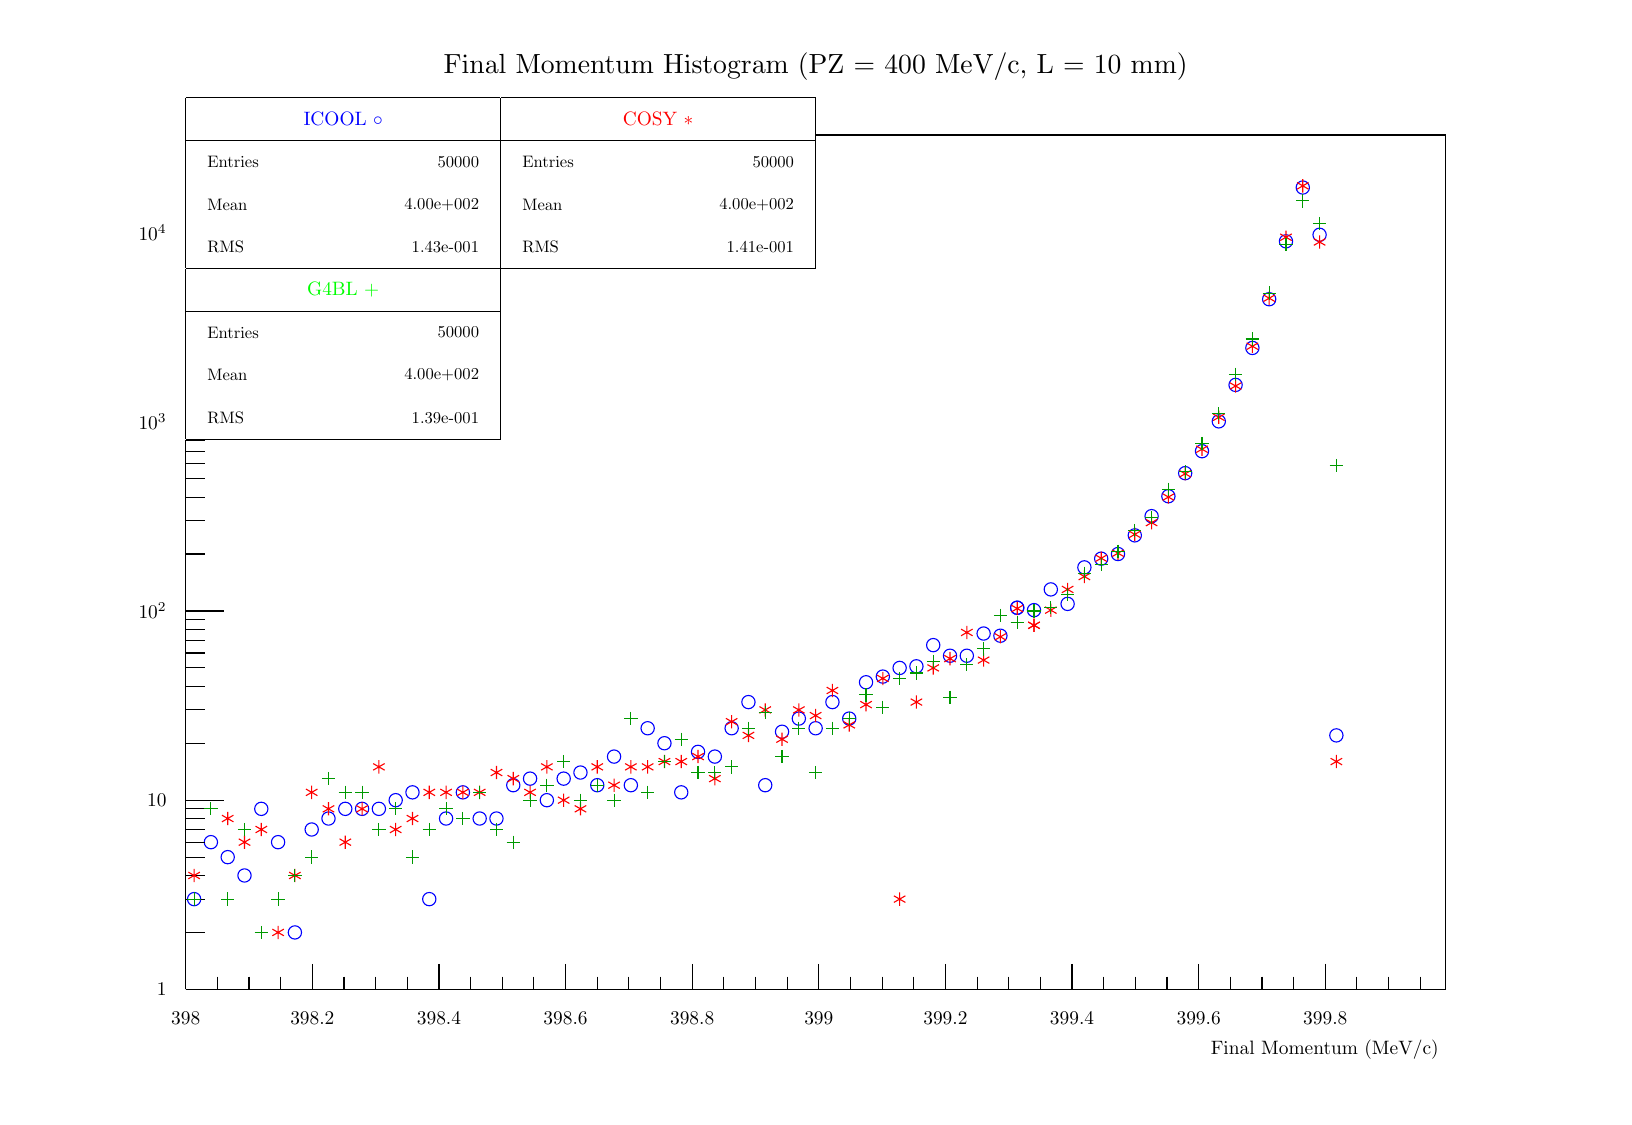
\begin{tikzpicture}
\definecolor{c}{rgb}{1,1,1};
\draw [color=c, fill=c] (0,0) rectangle (20,13.5632);
\draw [color=c, fill=c] (2,1.35632) rectangle (18,12.2069);
\definecolor{c}{rgb}{0,0,0};
\draw [c] (2,1.35632) -- (2,12.2069) -- (18,12.2069) -- (18,1.35632) -- (2,1.35632);
\definecolor{c}{rgb}{1,1,1};
\draw [color=c, fill=c] (2,1.35632) rectangle (18,12.2069);
\definecolor{c}{rgb}{0,0,0};
\draw [c] (2,1.35632) -- (2,12.2069) -- (18,12.2069) -- (18,1.35632) -- (2,1.35632);
\definecolor{c}{rgb}{0,0,1};
\foreach \P in
 {(2.10667,2.50282),(2.32,3.22618),(2.53333,3.03591),(2.74667,2.80304),(2.96,3.64932),(3.17333,3.22618),(3.38667,2.07968),(3.6,3.38705),(3.81333,3.5264),(4.02667,3.64932),(4.24,3.64932),(4.45333,3.64932),(4.66667,3.75927),(4.88,3.85874),(5.09333,2.50
282),(5.30667,3.5264),(5.52,3.85874),(5.73333,3.5264),(5.94667,3.5264),(6.16,3.94954),(6.37333,4.03307),(6.58667,3.75927),(6.8,4.03307),(7.01333,4.11041),(7.22667,3.94954),(7.44,4.31303),(7.65333,3.94954),(7.86667,4.6729),(8.08,4.48263),(8.29333,3.85
874),(8.50667,4.37268),(8.72,4.31303),(8.93333,4.6729),(9.14667,5.00524),(9.36,3.94954),(9.57333,4.62849),(9.78667,4.79582),(10,4.6729),(10.2133,5.00524),(10.4267,4.79582),(10.64,5.25691),(10.8533,5.32891),(11.0667,5.43886),(11.28,5.45953),(11.4933,5
.7286),(11.7067,5.59375),(11.92,5.59375),(12.1333,5.87583),(12.3467,5.84799),(12.56,6.20316)}{\draw[mark options={color=c,fill=c},mark size=2.402402pt,mark=o] plot coordinates {\P};}
\foreach \P in
 {(12.56,6.20316),(12.7733,6.17261),(12.9867,6.43603),(13.2,6.25216),(13.4133,6.71598),(13.6267,6.82655),(13.84,6.88559),(14.0533,7.12262),(14.2667,7.36625),(14.48,7.61933),(14.6933,7.91242),(14.9067,8.19146),(15.12,8.57038),(15.3333,9.03325),(15.546
7,9.50288),(15.76,10.1215),(15.9733,10.8567),(16.1867,11.54),(16.4,10.9398),(16.6133,4.5821)}{\draw[mark options={color=c,fill=c},mark size=2.402402pt,mark=o] plot coordinates {\P};}
\definecolor{c}{rgb}{1,1,1};
\draw [color=c, fill=c] (2,10.5115) rectangle (6,12.6816);
\definecolor{c}{rgb}{0,0,0};
\draw [c] (2,10.5115) -- (6,10.5115);
\draw [c] (6,10.5115) -- (6,12.6816);
\draw [c] (6,12.6816) -- (2,12.6816);
\draw [c] (2,12.6816) -- (2,10.5115);
\draw[color=blue](4,12.4103) node[scale=0.7, rotate=0]{ICOOL $\circ$};
\draw [c] (2,12.1391) -- (6,12.1391);
\draw [anchor= west] (2.2,11.8678) node[scale=0.6, rotate=0]{Entries };
\draw [anchor= east] (5.8,11.8678) node[scale=0.6, rotate=0]{ 50000};
\draw [anchor= west] (2.2,11.3253) node[scale=0.6, rotate=0]{Mean  };
\draw [anchor= east] (5.8,11.3253) node[scale=0.6, rotate=0]{ 4.00e+002};
\draw [anchor= west] (2.2,10.7828) node[scale=0.6, rotate=0]{RMS   };
\draw [anchor= east] (5.8,10.7828) node[scale=0.6, rotate=0]{ 1.43e-001};
\draw [c] (2,1.35632) -- (18,1.35632);
\draw [anchor= east] (18,0.596782) node[scale=0.7, rotate=0]{Final Momentum (MeV/c)};
\draw [c] (2,1.68184) -- (2,1.35632);
\draw [c] (2.40201,1.51908) -- (2.40201,1.35632);
\draw [c] (2.80402,1.51908) -- (2.80402,1.35632);
\draw [c] (3.20603,1.51908) -- (3.20603,1.35632);
\draw [c] (3.60804,1.68184) -- (3.60804,1.35632);
\draw [c] (4.01005,1.51908) -- (4.01005,1.35632);
\draw [c] (4.41206,1.51908) -- (4.41206,1.35632);
\draw [c] (4.81407,1.51908) -- (4.81407,1.35632);
\draw [c] (5.21608,1.68184) -- (5.21608,1.35632);
\draw [c] (5.61809,1.51908) -- (5.61809,1.35632);
\draw [c] (6.0201,1.51908) -- (6.0201,1.35632);
\draw [c] (6.42211,1.51908) -- (6.42211,1.35632);
\draw [c] (6.82412,1.68184) -- (6.82412,1.35632);
\draw [c] (7.22613,1.51908) -- (7.22613,1.35632);
\draw [c] (7.62814,1.51908) -- (7.62814,1.35632);
\draw [c] (8.03015,1.51908) -- (8.03015,1.35632);
\draw [c] (8.43216,1.68184) -- (8.43216,1.35632);
\draw [c] (8.83417,1.51908) -- (8.83417,1.35632);
\draw [c] (9.23618,1.51908) -- (9.23618,1.35632);
\draw [c] (9.63819,1.51908) -- (9.63819,1.35632);
\draw [c] (10.0402,1.68184) -- (10.0402,1.35632);
\draw [c] (10.4422,1.51908) -- (10.4422,1.35632);
\draw [c] (10.8442,1.51908) -- (10.8442,1.35632);
\draw [c] (11.2462,1.51908) -- (11.2462,1.35632);
\draw [c] (11.6482,1.68184) -- (11.6482,1.35632);
\draw [c] (12.0503,1.51908) -- (12.0503,1.35632);
\draw [c] (12.4523,1.51908) -- (12.4523,1.35632);
\draw [c] (12.8543,1.51908) -- (12.8543,1.35632);
\draw [c] (13.2563,1.68184) -- (13.2563,1.35632);
\draw [c] (13.6583,1.51908) -- (13.6583,1.35632);
\draw [c] (14.0603,1.51908) -- (14.0603,1.35632);
\draw [c] (14.4623,1.51908) -- (14.4623,1.35632);
\draw [c] (14.8643,1.68184) -- (14.8643,1.35632);
\draw [c] (15.2663,1.51908) -- (15.2663,1.35632);
\draw [c] (15.6683,1.51908) -- (15.6683,1.35632);
\draw [c] (16.0704,1.51908) -- (16.0704,1.35632);
\draw [c] (16.4724,1.68184) -- (16.4724,1.35632);
\draw [c] (16.4724,1.68184) -- (16.4724,1.35632);
\draw [c] (16.8744,1.51908) -- (16.8744,1.35632);
\draw [c] (17.2764,1.51908) -- (17.2764,1.35632);
\draw [c] (17.6784,1.51908) -- (17.6784,1.35632);
\draw [anchor=base] (2,0.908736) node[scale=0.7, rotate=0]{398};
\draw [anchor=base] (3.60804,0.908736) node[scale=0.7, rotate=0]{398.2};
\draw [anchor=base] (5.21608,0.908736) node[scale=0.7, rotate=0]{398.4};
\draw [anchor=base] (6.82412,0.908736) node[scale=0.7, rotate=0]{398.6};
\draw [anchor=base] (8.43216,0.908736) node[scale=0.7, rotate=0]{398.8};
\draw [anchor=base] (10.0402,0.908736) node[scale=0.7, rotate=0]{399};
\draw [anchor=base] (11.6482,0.908736) node[scale=0.7, rotate=0]{399.2};
\draw [anchor=base] (13.2563,0.908736) node[scale=0.7, rotate=0]{399.4};
\draw [anchor=base] (14.8643,0.908736) node[scale=0.7, rotate=0]{399.6};
\draw [anchor=base] (16.4724,0.908736) node[scale=0.7, rotate=0]{399.8};
\draw [c] (2,1.35632) -- (2,12.2069);
\draw [c] (2.48,1.35632) -- (2,1.35632);
\draw [anchor= east] (1.844,1.35632) node[scale=0.7, rotate=0]{1};
\draw [c] (2.24,2.07968) -- (2,2.07968);
\draw [c] (2.24,2.50282) -- (2,2.50282);
\draw [c] (2.24,2.80304) -- (2,2.80304);
\draw [c] (2.24,3.03591) -- (2,3.03591);
\draw [c] (2.24,3.22618) -- (2,3.22618);
\draw [c] (2.24,3.38705) -- (2,3.38705);
\draw [c] (2.24,3.52641) -- (2,3.52641);
\draw [c] (2.24,3.64932) -- (2,3.64932);
\draw [c] (2.48,3.75928) -- (2,3.75928);
\draw [anchor= east] (1.844,3.75928) node[scale=0.7, rotate=0]{10};
\draw [c] (2.24,4.48264) -- (2,4.48264);
\draw [c] (2.24,4.90577) -- (2,4.90577);
\draw [c] (2.24,5.206) -- (2,5.206);
\draw [c] (2.24,5.43887) -- (2,5.43887);
\draw [c] (2.24,5.62913) -- (2,5.62913);
\draw [c] (2.24,5.79) -- (2,5.79);
\draw [c] (2.24,5.92936) -- (2,5.92936);
\draw [c] (2.24,6.05227) -- (2,6.05227);
\draw [c] (2.48,6.16223) -- (2,6.16223);
\draw [anchor= east] (1.844,6.16223) node[scale=0.7, rotate=0]{$10^{2}$};
\draw [c] (2.24,6.88559) -- (2,6.88559);
\draw [c] (2.24,7.30872) -- (2,7.30872);
\draw [c] (2.24,7.60895) -- (2,7.60895);
\draw [c] (2.24,7.84182) -- (2,7.84182);
\draw [c] (2.24,8.03209) -- (2,8.03209);
\draw [c] (2.24,8.19296) -- (2,8.19296);
\draw [c] (2.24,8.33231) -- (2,8.33231);
\draw [c] (2.24,8.45522) -- (2,8.45522);
\draw [c] (2.48,8.56518) -- (2,8.56518);
\draw [anchor= east] (1.844,8.56518) node[scale=0.7, rotate=0]{$10^{3}$};
\draw [c] (2.24,9.28854) -- (2,9.28854);
\draw [c] (2.24,9.71168) -- (2,9.71168);
\draw [c] (2.24,10.0119) -- (2,10.0119);
\draw [c] (2.24,10.2448) -- (2,10.2448);
\draw [c] (2.24,10.435) -- (2,10.435);
\draw [c] (2.24,10.5959) -- (2,10.5959);
\draw [c] (2.24,10.7353) -- (2,10.7353);
\draw [c] (2.24,10.8582) -- (2,10.8582);
\draw [c] (2.48,10.9681) -- (2,10.9681);
\draw [anchor= east] (1.844,10.9681) node[scale=0.7, rotate=0]{$10^{4}$};
\draw [c] (2.24,11.6915) -- (2,11.6915);
\draw [c] (2.24,12.1146) -- (2,12.1146);
\definecolor{c}{rgb}{1,1,1};
\draw [color=c, fill=c] (2,10.5115) rectangle (6,12.6816);
\definecolor{c}{rgb}{0,0,0};
\draw [c] (2,10.5115) -- (6,10.5115);
\draw [c] (6,10.5115) -- (6,12.6816);
\draw [c] (6,12.6816) -- (2,12.6816);
\draw [c] (2,12.6816) -- (2,10.5115);
\draw[color=blue](4,12.4103) node[scale=0.7, rotate=0]{ICOOL $\circ$};
\draw [c] (2,12.1391) -- (6,12.1391);
\draw [anchor= west] (2.2,11.8678) node[scale=0.6, rotate=0]{Entries };
\draw [anchor= east] (5.8,11.8678) node[scale=0.6, rotate=0]{ 50000};
\draw [anchor= west] (2.2,11.3253) node[scale=0.6, rotate=0]{Mean  };
\draw [anchor= east] (5.8,11.3253) node[scale=0.6, rotate=0]{ 4.00e+002};
\draw [anchor= west] (2.2,10.7828) node[scale=0.6, rotate=0]{RMS   };
\draw [anchor= east] (5.8,10.7828) node[scale=0.6, rotate=0]{ 1.43e-001};
\draw (10,13.0816) node[scale=1, rotate=0]{Final Momentum Histogram (PZ = 400 MeV/c, L = 10 mm)};
\definecolor{c}{rgb}{1,0,0};
\foreach \P in
 {(2.10667,2.80304),(2.53333,3.5264),(2.74667,3.22618),(2.96,3.38705),(3.17333,2.07968),(3.38667,2.80304),(3.6,3.85874),(3.81333,3.64932),(4.02667,3.22618),(4.24,3.64932),(4.45333,4.18241),(4.66667,3.38705),(4.88,3.5264),(5.09333,3.85874),(5.30667,3.
85874),(5.52,3.85874),(5.73333,3.85874),(5.94667,4.11041),(6.16,4.03307),(6.37333,3.85874),(6.58667,4.18241),(6.8,3.75927),(7.01333,3.64932),(7.22667,4.18241),(7.44,3.94954),(7.65333,4.18241),(7.86667,4.18241),(8.08,4.24976),(8.29333,4.24976),(8.5066
7,4.31303),(8.72,4.03307),(8.93333,4.75643),(9.14667,4.5821),(9.36,4.90577),(9.57333,4.53355),(9.78667,4.90577),(10,4.83377),(10.2133,5.15246),(10.4267,4.7155),(10.64,4.97312),(10.8533,5.30546),(11.0667,2.50282),(11.28,5.00524),(11.4933,5.43886),(11.
7067,5.55713),(11.92,5.88947),(12.1333,5.53833),(12.3467,5.8338),(12.56,6.19307),(12.7733,5.98027)}{\draw[mark options={color=c,fill=c},mark size=2.402402pt,mark=asterisk] plot coordinates {\P};}
\foreach \P in
 {(12.7733,5.98027),(12.9867,6.17261),(13.2,6.43603),(13.4133,6.59919),(13.6267,6.83206),(13.84,6.89597),(14.0533,7.13502),(14.2667,7.28408),(14.48,7.60895),(14.6933,7.90459),(14.9067,8.21654),(15.12,8.62204),(15.3333,9.01916),(15.5467,9.52432),(15.7
6,10.1343),(15.9733,10.9086),(16.1867,11.5612),(16.4,10.848),(16.6133,4.24976)}{\draw[mark options={color=c,fill=c},mark size=2.402402pt,mark=asterisk] plot coordinates {\P};}
\definecolor{c}{rgb}{1,1,1};
\draw [color=c, fill=c] (6,10.5115) rectangle (10,12.6816);
\definecolor{c}{rgb}{0,0,0};
\draw [c] (6,10.5115) -- (10,10.5115);
\draw [c] (10,10.5115) -- (10,12.6816);
\draw [c] (10,12.6816) -- (6,12.6816);
\draw [c] (6,12.6816) -- (6,10.5115);
\draw [color=red](8,12.4103) node[scale=0.7, rotate=0]{COSY $*$};
\draw [c] (6,12.1391) -- (10,12.1391);
\draw [anchor= west] (6.2,11.8678) node[scale=0.6, rotate=0]{Entries };
\draw [anchor= east] (9.8,11.8678) node[scale=0.6, rotate=0]{ 50000};
\draw [anchor= west] (6.2,11.3253) node[scale=0.6, rotate=0]{Mean  };
\draw [anchor= east] (9.8,11.3253) node[scale=0.6, rotate=0]{ 4.00e+002};
\draw [anchor= west] (6.2,10.7828) node[scale=0.6, rotate=0]{RMS   };
\draw [anchor= east] (9.8,10.7828) node[scale=0.6, rotate=0]{ 1.41e-001};
\definecolor{c}{rgb}{1,1,1};
\draw [color=c, fill=c] (6,10.5115) rectangle (10,12.6816);
\definecolor{c}{rgb}{0,0,0};
\draw [c] (6,10.5115) -- (10,10.5115);
\draw [c] (10,10.5115) -- (10,12.6816);
\draw [c] (10,12.6816) -- (6,12.6816);
\draw [c] (6,12.6816) -- (6,10.5115);
\draw [color=red](8,12.4103) node[scale=0.7, rotate=0]{COSY $*$};
\draw [c] (6,12.1391) -- (10,12.1391);
\draw [anchor= west] (6.2,11.8678) node[scale=0.6, rotate=0]{Entries };
\draw [anchor= east] (9.8,11.8678) node[scale=0.6, rotate=0]{ 50000};
\draw [anchor= west] (6.2,11.3253) node[scale=0.6, rotate=0]{Mean  };
\draw [anchor= east] (9.8,11.3253) node[scale=0.6, rotate=0]{ 4.00e+002};
\draw [anchor= west] (6.2,10.7828) node[scale=0.6, rotate=0]{RMS   };
\draw [anchor= east] (9.8,10.7828) node[scale=0.6, rotate=0]{ 1.41e-001};
\definecolor{c}{rgb}{0,0.6,0};
\foreach \P in
 {(2.10667,2.50282),(2.32,3.64932),(2.53333,2.50282),(2.74667,3.38705),(2.96,2.07968),(3.17333,2.50282),(3.38667,2.80304),(3.6,3.03591),(3.81333,4.03307),(4.02667,3.85874),(4.24,3.85874),(4.45333,3.38705),(4.66667,3.64932),(4.88,3.03591),(5.09333,3.3
8705),(5.30667,3.64932),(5.52,3.5264),(5.73333,3.85874),(5.94667,3.38705),(6.16,3.22618),(6.37333,3.75927),(6.58667,3.94954),(6.8,4.24976),(7.01333,3.75927),(7.22667,3.94954),(7.44,3.75927),(7.65333,4.79582),(7.86667,3.85874),(8.08,4.24976),(8.29333,
4.53355),(8.50667,4.11041),(8.72,4.11041),(8.93333,4.18241),(9.14667,4.6729),(9.36,4.87039),(9.57333,4.31303),(9.78667,4.6729),(10,4.11041),(10.2133,4.6729),(10.4267,4.79582),(10.64,5.09604),(10.8533,4.93999),(11.0667,5.30546),(11.28,5.37429),(11.493
3,5.51918),(11.7067,5.06664),(11.92,5.47979),(12.1333,5.68005),(12.3467,6.1087),(12.56,6.01689)}{\draw[mark options={color=c,fill=c},mark size=2.402402pt,mark=+] plot coordinates {\P};}
\foreach \P in
 {(12.56,6.01689),(12.7733,6.16222),(12.9867,6.20316),(13.2,6.36974),(13.4133,6.63959),(13.6267,6.75218),(13.84,6.92149),(14.0533,7.18319),(14.2667,7.3463),(14.48,7.70841),(14.6933,7.92791),(14.9067,8.2897),(15.12,8.66654),(15.3333,9.16927),(15.5467,
9.61631),(15.76,10.1991),(15.9733,10.8192),(16.1867,11.3705),(16.4,11.0823),(16.6133,8.011)}{\draw[mark options={color=c,fill=c},mark size=2.402402pt,mark=+] plot coordinates {\P};}
\definecolor{c}{rgb}{1,1,1};
\draw [color=c, fill=c] (2,8.34138) rectangle (6,10.5115);
\definecolor{c}{rgb}{0,0,0};
\draw [c] (2,8.34138) -- (6,8.34138);
\draw [c] (6,8.34138) -- (6,10.5115);
\draw [c] (6,10.5115) -- (2,10.5115);
\draw [c] (2,10.5115) -- (2,8.34138);
\draw [color=green](4,10.2402) node[scale=0.7, rotate=0]{G4BL $+$};
\draw [c] (2,9.96897) -- (6,9.96897);
\draw [anchor= west] (2.2,9.6977) node[scale=0.6, rotate=0]{Entries };
\draw [anchor= east] (5.8,9.6977) node[scale=0.6, rotate=0]{ 50000};
\draw [anchor= west] (2.2,9.15517) node[scale=0.6, rotate=0]{Mean  };
\draw [anchor= east] (5.8,9.15517) node[scale=0.6, rotate=0]{ 4.00e+002};
\draw [anchor= west] (2.2,8.61264) node[scale=0.6, rotate=0]{RMS   };
\draw [anchor= east] (5.8,8.61264) node[scale=0.6, rotate=0]{ 1.39e-001};
\definecolor{c}{rgb}{1,1,1};
\draw [color=c, fill=c] (2,8.34138) rectangle (6,10.5115);
\definecolor{c}{rgb}{0,0,0};
\draw [c] (2,8.34138) -- (6,8.34138);
\draw [c] (6,8.34138) -- (6,10.5115);
\draw [c] (6,10.5115) -- (2,10.5115);
\draw [c] (2,10.5115) -- (2,8.34138);
\draw [color=green](4,10.2402) node[scale=0.7, rotate=0]{G4BL $+$};
\draw [c] (2,9.96897) -- (6,9.96897);
\draw [anchor= west] (2.2,9.6977) node[scale=0.6, rotate=0]{Entries };
\draw [anchor= east] (5.8,9.6977) node[scale=0.6, rotate=0]{ 50000};
\draw [anchor= west] (2.2,9.15517) node[scale=0.6, rotate=0]{Mean  };
\draw [anchor= east] (5.8,9.15517) node[scale=0.6, rotate=0]{ 4.00e+002};
\draw [anchor= west] (2.2,8.61264) node[scale=0.6, rotate=0]{RMS   };
\draw [anchor= east] (5.8,8.61264) node[scale=0.6, rotate=0]{ 1.39e-001};
\end{tikzpicture}
